\documentclass{article}
\usepackage[margin=2.5cm, top=4cm, headheight=25pt]{geometry}
\usepackage{amsmath, amssymb, enumitem, fancyhdr, graphicx}
\usepackage[indent=20pt]{parskip}
\usepackage[hidelinks]{hyperref}
\usepackage{xcolor}
\usepackage{listings}
\usepackage{subcaption}
\usepackage{url}
\usepackage[most]{tcolorbox}
\usepackage{lastpage}

\tcbuselibrary{listingsutf8} % Support for lstlistings within tcolorbox

\newtcolorbox[auto counter, number within=section]{question}[1][]{%
    colframe=gray!80,                      % Dark gray frame
    colback=gray!5,                       % Light gray background
    coltitle=black,                        % Black title
    title=\textbf{Question~\thetcbcounter}, % Bold title
    fonttitle=\bfseries\large,             % Subtle title font size
    rounded corners,                   % Slightly more rounded corners
    boxrule=0.25mm,                         % Thinner border for a sleek look
    enhanced,                              % Enhanced box features
    attach boxed title to top left={xshift=2mm, yshift=-2mm},
    boxed title style={colframe=gray!80, colback=gray!5, boxrule=0.25mm},
    % Title styling
    #1
}

\bibliographystyle{IEEEtran}
\graphicspath{{./images/}}

% -- Custom Variables --
\def\me{Rajdeep Gill 7934493}
\def\course{COURSE CODE}
\def\labsection{SECTION}
\def\labno{LABNO}
\def\title{TITLE}

% -- Styling for code snippets --
\lstset{
    basicstyle=\ttfamily\small,           % Basic font style
    keywordstyle=\color{blue},            % Keywords color
    commentstyle=\color{gray},            % Comments color
    stringstyle=\color{teal},             % Strings color
    numbers=left,                         % Line numbers on the left
    numberstyle=\tiny\color{gray},        % Line number style
    stepnumber=1,                         % Line number step
    numbersep=10pt,                       % Space between line numbers and code
    backgroundcolor=\color{lightgray!10}, % Background color
    frame=single,                         % Adds a frame around the code
    breaklines=true,                      % Line breaking for long lines
    captionpos=b,                         % Caption position
    showspaces=false,                     % Don't show spaces
    showstringspaces=false                % Don't show spaces in strings
}
\renewcommand{\lstlistingname}{Code Snippet}

\renewcommand{\arraystretch}{1.2} % For less-ugly tables
\setlength\parindent{0pt}

%----- Samples 
% Questions:
%   \begin{question}[title=Custom Question Title]
%       Question details
%   \end{question}

% Tables:
%   \begin{table}[htbp]
%       \centering
%       \caption{Table Caption}
%       \begin{tabular}{ll}
%           \toprule
%           \textbf{Column 1} & \textbf{Column 2} \\
%           \midrule
%           Row 1 & Row 2 \\
%           Row 3 & Row 4 \\
%           \bottomrule
%       \end{tabular}
%   \end{table} 

% Figures:
%   Single figure:
%       \begin{figure}[htbp]
%           \centering
%           \includegraphics[width=0.5\textwidth]{example-image}
%           \caption{Figure Caption}
%       \end{figure}
%   Multiple figures:
%       \begin{figure}[htbp]
%           \centering
%           \begin{subfigure}[b]{0.5\textwidth}
%               \includegraphics[width=\textwidth]{example-image-a}
%               \caption{First subfigure}
%           \end{subfigure}
%           \begin{subfigure}[b]{0.5\textwidth}
%               \includegraphics[width=\textwidth]{example-image-b}
%               \caption{Second subfigure}
%           \end{subfigure}
%           \caption{Main figure}
%       \end{figure}

\begin{document}

% --------------------------------------------------------------------------------
% TITLE
% --------------------------------------------------------------------------------

\begin{center}
    \huge \title

    \vspace{2mm}
    \hrule

    \vspace{4mm}
    \large \me

    \vspace{2mm}
    \large \course~\labsection

    \vspace{2mm}
    \today
\end{center}

\vspace{4mm}

% --------------------------------------------------------------------------------
% END TITLE
% --------------------------------------------------------------------------------

\newpage

\tableofcontents

\vspace{1cm}
\newpage

\pagestyle{fancy}
\fancyhead[L]{\large Lab \labno}
\fancyhead[R]{\large \me}

\fancyfoot[C]{Page \thepage~of~\pageref{LastPage}}

% --------------------------------------------------------------------------------
% BODY
% --------------------------------------------------------------------------------
\section{Wireshark Lab: Getting Started}
\begin{enumerate}
    \item The different protocols that appear in the protocol column in the unfiltered packet-listing window are:
    \begin{itemize}
        \item UDP, TCP, DNS, HTTP, ICMPv6, TLSv1.2, LLC, TLSv1.3,
    \end{itemize}

    Some of these packets can be see in \autoref{fig:p1_1}.

    \begin{figure}[ht!]
        \centering
        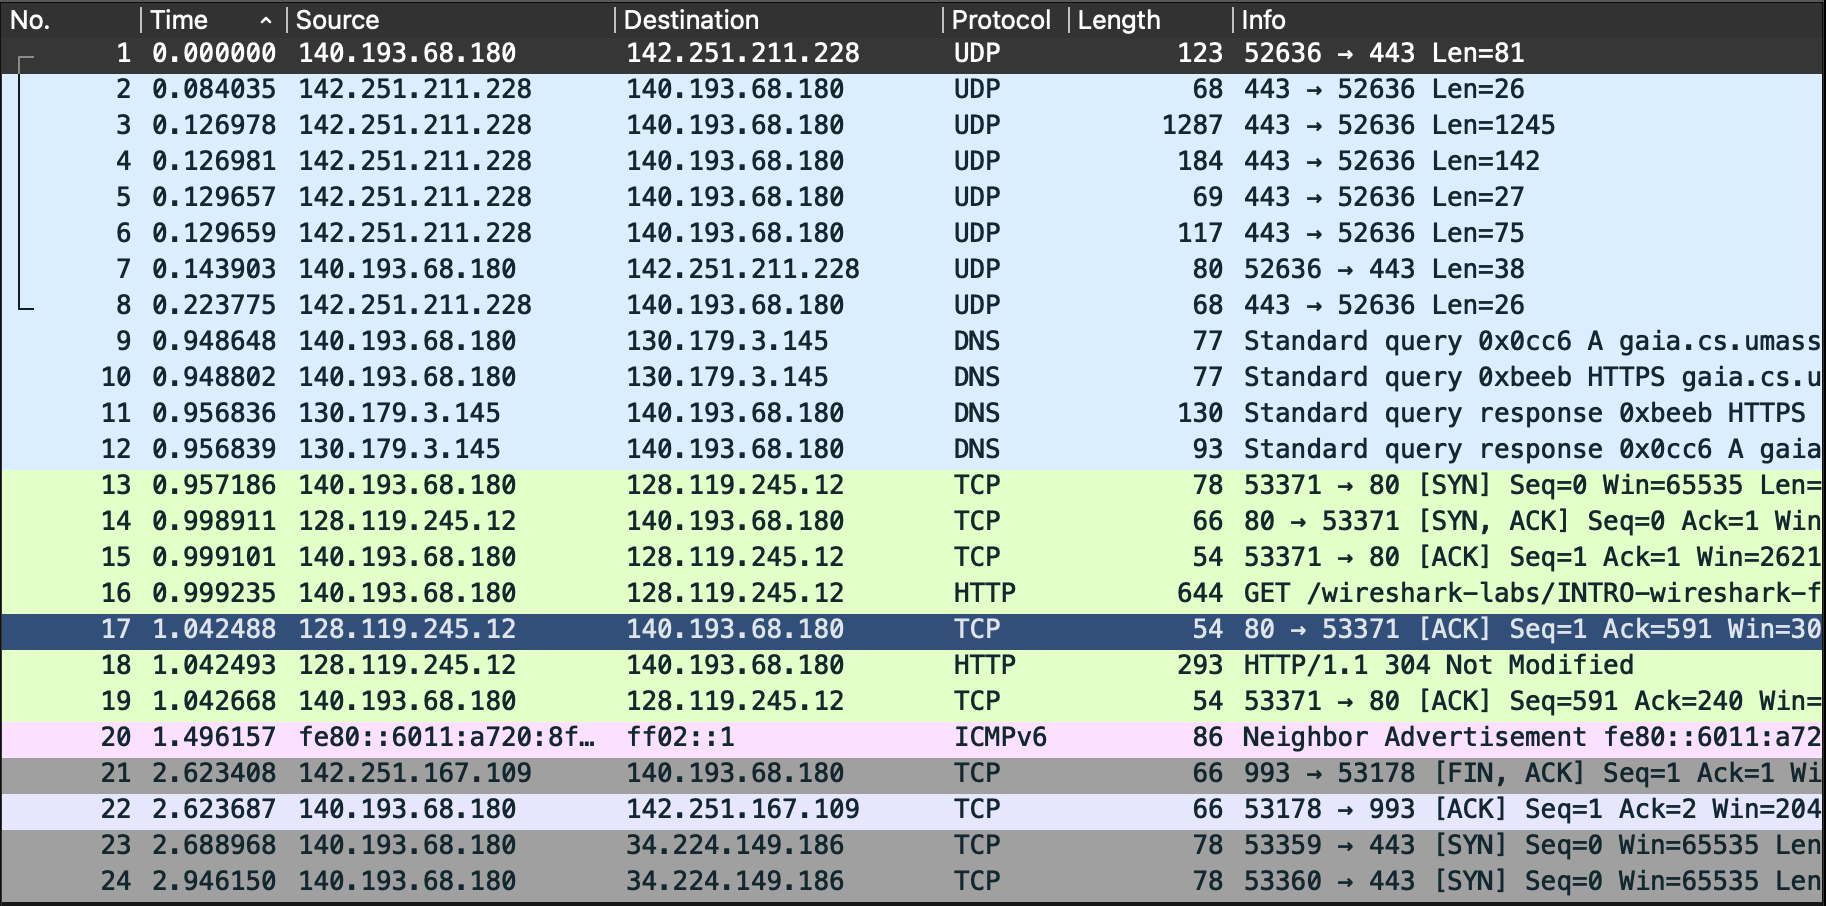
\includegraphics[width=0.8\textwidth]{p1_1}
        \caption{Packet-listing window}
        \label{fig:p1_1}
    \end{figure}


    \item The time taken for when the HTTP GET message was sent to when the HTTP OK reply was recieved was 0.04264 seconds. This was calculated by subtracting the time the HTTP GET message was sent from the time the HTTP OK reply was recieved. This can be seen in \autoref{fig:p1_2}.

    \begin{figure}[ht!]
        \centering
        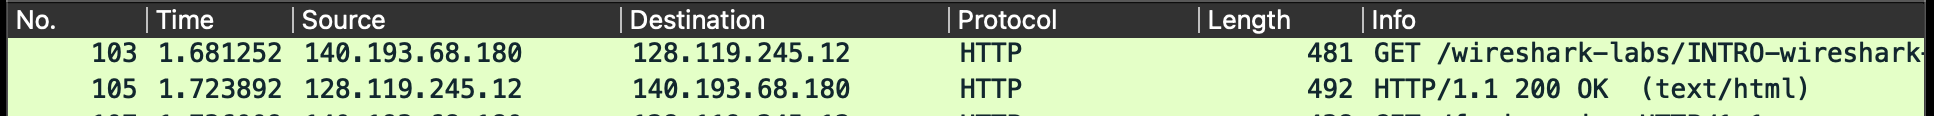
\includegraphics[width=0.8\textwidth]{p1_2}
        \caption{Time taken for HTTP GET message to HTTP OK reply}
        \label{fig:p1_2}
    \end{figure}

    \item The Internet address of the gaia.cs.umass.edu is 128.119.245.12 and the Internet address of my computer is 140.193.68.100. These addresses are sseen in \autoref{fig:p1_2}.
    
    \item Making 20 different requests and finding the delay between the HTTP GET message and the HTTP OK reply, the average delay was 0.08513 seconds. The plot of the 20 different requests can be seen in \autoref{fig:p1_3}.
    
    \begin{figure}[ht!]
        \centering
        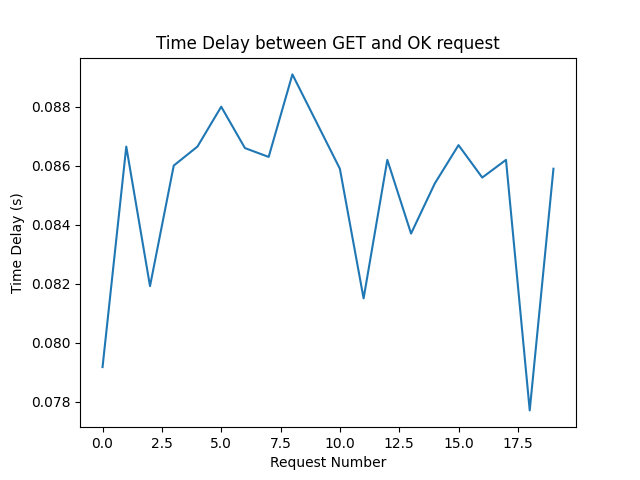
\includegraphics[width=0.8\textwidth]{p1_3}
        \caption{20 different requests}
        \label{fig:p1_3}
    \end{figure}
\end{enumerate}

\newpage
\section{Wireshark Lab: HTTP}

\begin{enumerate}
    \item The browser is running HTTP version 1.1 and so is the server. This can be deduced from the GET and OK requests both having HTTP/1.1 in the info column.
    \item Todo
    \item The IP address of my computer is 140.193.68.100 and the gaia.cs.umass.edu server is 128.119.245.12. This can be seen in the GET request and OK response.
    \item The status code returned by the server is 200. This can be seen in the info column of the OK request.
    \item The file was last modified at: . This can be seen in OK response from the server in the Hypertext Transfer Protocol section.
    \item 576 bytes of content was returned to the browser, and can be seen in the frame section of the GET response.
    \item perhaps
\end{enumerate}


\section{The HTTP CONDITIONAL GET/response interaction}
\begin{enumerate}
    \setcounter{enumi}{7}
    \item The first HTTP GET request does not have an If-Modified-Since header. 
    \item The server does return the contents of the file as we can see the content length of is 371.
    \item Inspecting the second HTTP GET request, we do see an If-Modified-Since header. The info followed by the header is ``If-Modified-Since: Tue, 23 Sep 2003 05:35:00 GMT$\backslash$r$\backslash$n''. This can be seen in the Hypertext Transfer Protocol section of the GET request.
    \item The HTTP status code of is 304 with a response phrase of Not Modified. The server did not explicitly return the contents of the file as the browser already had the file cached. There is also no content length in the response.
\end{enumerate}

\section{Retrieving Long Documents}
\begin{enumerate}
    \setcounter{enumi}{11}
    \item 1 HTTP GET request messages were sent by the browser. 
    \item 5 TCP segments were needed to carry the single HTTP response message.
    \item The status code and phrase associated with the response to the HTTP GET request is 200 OK.
    \item There are 3 packets with status lines stating a continuation. 
\end{enumerate}

\section{HTML Documents with Embedded Objects}

\begin{enumerate}
    \setcounter{enumi}{15}
    \item 3 HTTP GET request messages were sent by the browser. One for the html and the other two for the image. The internet address of the first request was: 128.119.245.12, the second request was: 165.193.123.218 and the third request was: 134.241.6.82.
    \item The two images were done in parallel as the browser sent the request for the two images before any of the responses were received. In the packet listing window we see that the requests were both made before any of the responses were received.
\end{enumerate}

\section{HTTP Authentication}

\begin{enumerate}
    \setcounter{enumi}{17}
    \item In the initial HTTP GET request, the server responseds with a 401 code and a message of Authorization Required. 
    \item The new field in the second HTTP GET request is the Authorization field. It is a basic authentication field with the value encoded in base64.
\end{enumerate}

\section{Additional Questions}
\begin{enumerate}
    \item In the TCP/IP stack, HTTP belongs in the application layer.
    \item The underlying transport layer protocol used by TCP is IP.
    \item The HTTP response for a successful request is 200 OK.
    \item When a file exceeds the payload size of a single packet, the file is split into multiple TCP segments and are sent individually. The segments are then reassembled at the destination.
    \item The components of the HTTP status line are the status code and the status phrase.
    \item The encoding method used in HTTP authentication is base64.
    \item Basic authentication is not secure as base64 can be easily decoded, allowing the information in the header to be read. If it contains sensitive information, it can be easily stolen.l
\end{enumerate}

% --------------------------------------------------------------------------------
% END BODY
% --------------------------------------------------------------------------------

\end{document}
